\documentclass[../../Report.tex]{subfiles}
\graphicspath{{\subfix{../../images/}}}
\begin{document}
    \textbf{Thermoluminescence Dosimetry (TLD)} is a technique used to measure and assess radiation doses by exploiting 
    the thermoluminescent properties of certain materials. It is widely employed in various fields, including medical 
    radiation therapy, industrial radiation safety, environmental monitoring, and personal dosimetry.

    The basic principle of thermoluminescence dosimetry involves the use of thermoluminescent materials, which are 
    crystalline or amorphous substances capable of storing energy when exposed to ionizing radiation. These materials 
    can be in the form of powders, pellets, or chips. Common thermoluminescent materials include lithium fluoride ($LiF$), 
    calcium fluoride ($CaF_2$), and aluminum oxide ($Al_2O_3:C$). A Thermoluminescence Dosimeter is shown in figure\ref{fig:Dosimeter}

    \begin{Figure}
        \centering
        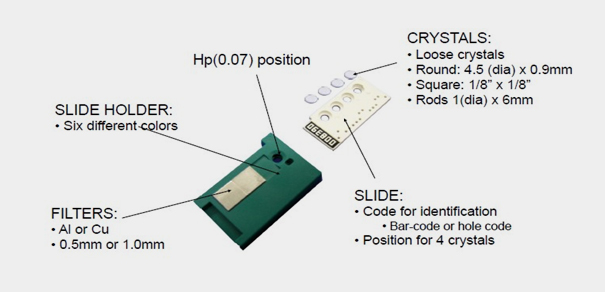
\includegraphics[width=0.8\linewidth]{Dosimeter.jpg}
        \captionof{figure}{A thermoluminescent dosimeter \cite{u6}}
        \label{fig:Dosimeter}
    \end{Figure}

    \subsubsection*{\large Thermoluminescence}
        Thermoluminescence (TL) is a luminescence phenomenon\cite{a6} of an insulator or semiconductor which can be observed when
        the solid is thermally stimulated. In order for a material to be thermoluminous, it must first be an insulator 
        or a semiconductor because metals do not show thermoluminescence. Secondly, energy must have been absorbed by 
        the substance at some point while it was exposed to ionising radiation. Thirdly, heating the material causes the 
        luminescence emission to occur. Thus, a thermoluminescent material is one that, when subjected to ionising 
        radiation, absorbs some energy that is then stored. When the substance is later heated, the accumulated energy is 
        released in the form of luminescence.\cite{b1}
        
        There are many models that explain the phenomenon of thermoluminescence\cite{b5}, one such model is the one 
        trapping—one recombination centre model\cite{b2} that uses the energy band theory of solids.The majority of the 
        electrons in an ideal crystalline semiconductor or insulator are found in the valence band. The conduction band, 
        which is above the valence band and is separated from it by the so-called forbidden band gap (separated by energy $E_g$ ), 
        is the highest band that electrons can inhabit. However, when a crystal has structural flaws or the lattice 
        contains impurities, it is possible for electrons to have energies that are not permitted in a perfect crystal.
        In a simple TL model two levels are assumed, one situated below the bottom of the conduction band and the other 
        situated above the top of the valence band as shown in figure \ref{fig:BandDiagram}. 

        \begin{Figure}
            \centering
            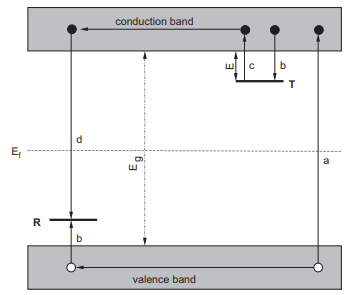
\includegraphics[width=0.5\linewidth]{BandDiagram.png}
            \captionof{figure}{Energy band model showing the electronic transitions in a TL material according to a 
            simple two-level model.\cite{a6}}
            \label{fig:BandDiagram}
        \end{Figure}
        
        The highest level is situated above the equilibrium Fermi level ($E_f$) and thus empty in the equilibrium state, 
        i.e. before the exposure to radiation and the creation of electrons and holes. It is therefore a potential 
        electron trap. The other level is a potential hole trap and can function as a recombination centre. 
        The absorption of radiant energy with $h \> E_g$ results in ionisation of valence electrons, producing 
        energetic electrons and holes which will, after thermalisation, produce free electrons in the conduction 
        band and free holes in the valence band. The free charge carriers recombine with each other or become trapped.

        An amount of energy will be generated in the case of direct recombination, which may stimulate a luminescent 
        centre (which might coincide with the recombination centre). Under the influence of light emission, the 
        luminescent centre relaxes (returns to the ground state).  However, in semiconductors and insulators a
        certain percentage of the charge carriers is trapped. As the free electrons and holes are created and annihilated
        in pairs, there must be an equal population of trapped holes Because the normal equilibrium Fermi level $E_f$ is
        situated below level T and above level R (as shown in figure \ref{fig:BandDiagram}), these populations of
        trapped electrons and holes represent a non-equilibrium state.

        By increasing the temperature of the TL material above $T_0$, the return to equilibrium can be accelerated. 
        The likelihood of detrapping will rise as a result, and the electrons will then be liberated from the trap and 
        enter the conduction band. Until it undergoes recombination at the recombination centre R, the charge carrier 
        migrates through the crystal's conduction band. In the simple model this recombination centre is a luminescent
        centre where the recombination of the electron and hole leaves the centre in one of the higher excited states. 
        Return to the ground state is coupled with the emission of light quanta, which give rise to the phenomena of 
        \textbf{Thermoluminescence}.

    \subsubsection*{\large Process of Thermoluminescence Dosimetry}
        The TLD typically involves the following steps:
        \begin{enumerate}
            \item \textbf{Pre-Irradiation: } The thermoluminescent material is first subjected to a controlled 
            pre-irradiation process. This step ensures that any residual luminescence from previous radiation 
            exposures is removed, allowing the material to return to its baseline state.

            \item \textbf{Irradiation: } The pre-irradiated thermoluminescent material is then exposed to ionizing 
            radiation. The type of radiation and its energy will depend on the specific application and purpose of 
            the dosimetry measurement.

            \item \textbf{Post-Irradiation: } After irradiation, the thermoluminescent material retains energy in the 
            form of trapped electrons within defects or lattice imperfections. The sample is carefully protected from 
            any light exposure to prevent the release of the stored energy prematurely.

            \item \textbf{Heating Process: } When the thermoluminescent material is heated, the trapped electrons are 
            released from their energy states and recombine with the trapped holes, resulting in the emission of light 
            in the form of thermoluminescence. The emitted light is proportional to the radiation dose received by the 
            material.

            \item \textbf{Light Detection: } The emitted thermoluminescent light is detected using specialized 
            photomultiplier tubes, photodiodes, or other light-detecting devices. The detected light signal is then 
            converted into an electrical signal for further analysis.

            \item \textbf{Analysis and Dose Calculation: } The electrical signal is analyzed to determine the intensity 
            or luminescent response of the thermoluminescent material. This response is correlated with a calibration 
            curve or conversion factors established through calibration with known radiation doses. By comparing the 
            luminescent response to the calibration curve, the radiation dose received by the material can be determined.

        \end{enumerate}

    \subsubsection*{\large Applications of TLD}
        Thermoluminescence dosimetry (TLD) has numerous applications in various fields where accurate measurement of 
        radiation doses is essential. Some of the key applications of thermoluminescence dosimetry are:

        \begin{itemize}
            \item \textbf{Radiation Therapy: } In medical radiation therapy, TLD is used to measure the radiation dose 
            delivered to patients during treatments such as external beam radiation therapy or brachytherapy. 
            TLD allows for precise and reliable dose verification, ensuring that the prescribed radiation dose is 
            accurately delivered to the target area while minimizing exposure to healthy tissues.

            \item \textbf{Occupational Radiation Monitoring: } TLD is extensively used in industries involving radiation 
            sources, such as nuclear power plants, radiography facilities, and research laboratories. Workers who are 
            potentially exposed to ionizing radiation wear TLD badges or rings, which contain TLD materials. These 
            dosimeters are then analyzed to assess the radiation dose received by the workers, ensuring compliance with 
            safety regulations and maintaining a safe working environment.

            \item \textbf{Environmental Radiation Monitoring: } TLD is employed in environmental radiation monitoring 
            to assess radiation levels in the environment, including soil, air, and water. It helps identify potential 
            sources of radiation and monitor any changes or increases in radiation levels that could pose risks to human 
            health or the environment. TLD is particularly valuable in assessing long-term exposure and cumulative dose 
            assessments in environmental studies.

            \item \textbf{Personal Dosimetry: } TLD is used in personal dosimetry to measure individual radiation 
            exposure in various settings. This includes personnel working with radiation sources in nuclear facilities, 
            research laboratories, and industrial settings. TLD badges or rings worn by individuals capture their 
            radiation exposure, which can be analyzed to assess dose levels and ensure compliance with safety 
            regulations.

            \item \textbf{Radiation Protection: } TLD is employed in the design and evaluation of radiation shielding 
            materials and techniques. It allows for the measurement of radiation doses behind shielding materials to 
            ensure their effectiveness in reducing exposure. TLD is also used in quality assurance tests for radiation 
            protection equipment, such as lead aprons and protective barriers, to verify their performance and ensure 
            proper shielding.

            \item \textbf{Radiation Emergency Response: } In the event of a radiological incident or accident, 
            TLD can be used to assess the radiation doses received by affected individuals. TLD badges or rings can be 
            distributed to emergency responders and workers involved in recovery operations, providing valuable data 
            on their radiation exposure and guiding appropriate medical interventions.

            \item \textbf{Archaeological Dating: } TLD is utilized in archaeological dating to determine the age of 
            ancient artifacts and geological samples. By measuring the thermoluminescence emitted from the material, 
            the accumulated radiation dose can be estimated, providing insights into the time since the material was 
            last heated or exposed to sunlight.

        \end{itemize}

    Thermoluminescence dosimetry offers several advantages, including high sensitivity, wide dynamic range, and 
    excellent tissue-equivalent properties. It is capable of measuring both high and low radiation doses, making it 
    suitable for various applications. Additionally, TLD materials have good reproducibility and stability, allowing 
    for reliable and accurate dose measurements over time.
\end{document}











